% !TEX root = ./main.tex
\documentclass[a4paper]{article}
% Course language: use [english] or [german].
\usepackage[german]{ajnotes}
\title{\textbf{Betriebwirtschaftslehre — Unternehmensbewertung und Managementwissenschaften}}
\begin{document}
    \maketitle
    \textit{siehe Folien inkl. Lösungen} \url{https://lms.uzh.ch/auth/RepositoryEntry/17910989063/CourseNode/82357896275733}
    \section{Eigenmittelbeschaffung (Eigenkapital)}
    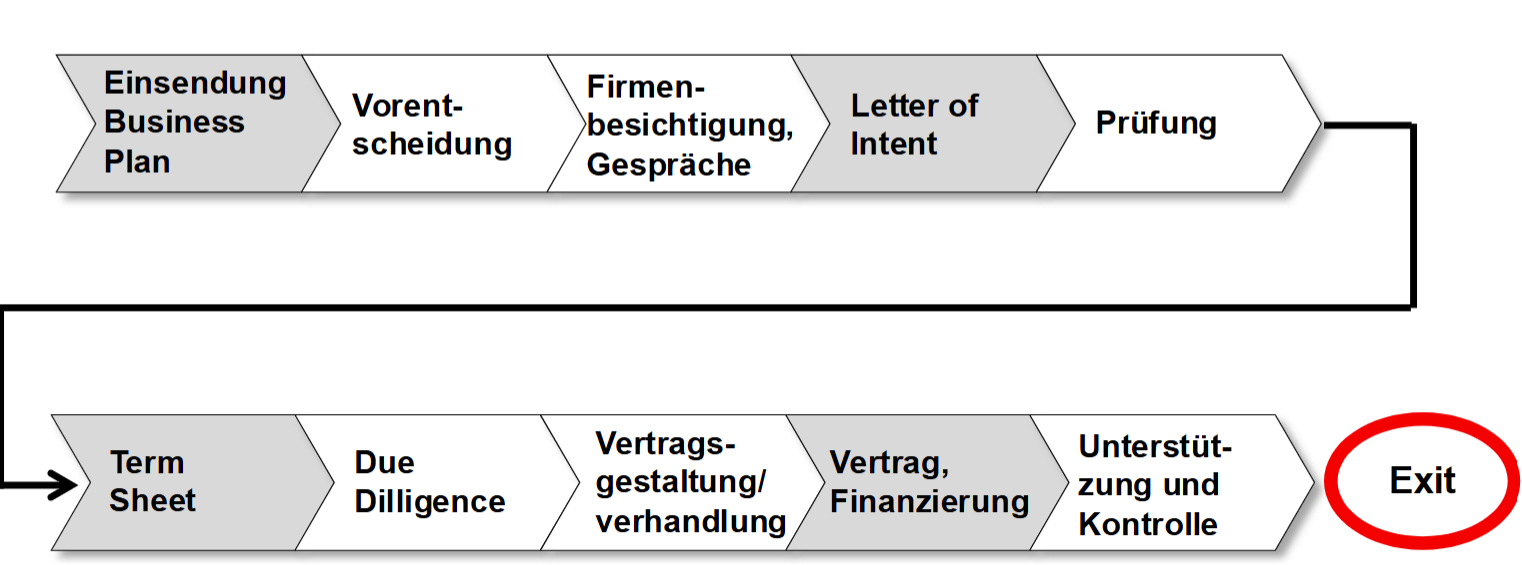
\includegraphics[width=\textwidth,height=0.7\textheight,keepaspectratio]{figures/Eigenmittel.png}

    \subsection{Letter of Intent}
    Ein nicht verbindlicher Brief zur Festhaltung der grundsätzlichen Absichten.
    \begin{itemize}
        \item Hauptthema: Erste Eckpunkte und offene Fragen, z.B. Einfluss des Investors und Berichtspflichten.
        \item Parteien: Investor und Unternehmen bzw. dessen Gründer.
        \item Ziel: Gemeinsames Interesse festhalten und die weiteren Verhandlungen vorbereiten.
    \end{itemize}

    \subsection{Term Sheet}
    \begin{itemize}
        \item Hauptthema: Wesentliche Investitionsbedingungen, etwa Bewertung, Investitionssumme, Beteiligung und Rechte.
        \item Ziel: Eine gemeinsame Grundlage für die Due Diligence und die Ausarbeitung der Verträge schaffen.
    \end{itemize}

    \subsection{Due Diligence}
    \begin{itemize}
        \item Hauptthema: Prüfung des Unternehmens und möglicher finanzieller, rechtlicher oder geschäftlicher Risiken.
        \item Ziel: Angaben und Risiken beurteilen und eine fundierte Investitionsentscheidung treffen.
    \end{itemize}
    \subsection{Vertrag und Finanzierung}
    \begin{itemize}
        \item Hauptthema: Verbindliche Regelung der Investition und Auszahlung des Kapitals.
        \item Ziel: Bedingungen rechtlich festhalten und die vereinbarte Finanzierung umsetzen.
    \end{itemize}
    \section{Bewertungsmethoden}

    \subsection{Funktion}
    \begin{itemize}
        \item Welcher Anteil des Unternehmens gehört den Investoren?
        \begin{itemize}
            \item Anteil muss also in Bezug zur Anlage des Investors im Verhältnis zum Unternehmenswert (Kapitalwert) berechnet werden.
            \item $\frac{Anlage}{Unternehmenswert*}$
        \end{itemize}
        \item Welche Rendite wird aus der Investition erwartet.
    \end{itemize}

    \subsection{Multiplikator Methode}
    \begin{itemize}
        \item Per Vergleich mit etablierten Firmen, eigene Wert sollte eine Fraktion des Referenzunternehmens entsprechen
        \item Abhängig der Qualität Unternehmensdaten
        \item Vorallem bei innovativen Startups ist ein Vergleich zu einem Referenzunternehmen schwierig, da diese oft nicht vorhanden sind. 
    \end{itemize}
    
    \subsection{Discounted Cashflow Methode (DCF)}
    \begin{itemize}
        \item Eignet sich für jede Art von Unternehmen
        \item Berechnung anhand von erwarteten Geldflüsse (Cashflows)
        \item Zukunftgerichtetes Verfahren\footnote{Das Gebrauchswert des Kapitals ist die zukünftige Selbstverwertung. }
    \end{itemize}

    \textbf{Berechnung:}
    \begin{itemize}
        \item $100 \cdot (1+r)^t$ = Zukünftige Mengegeld nach jährlichen Verzinsung (r) und Anzahl Jahre (t)
        \item Diskontierung ist die Mengegeld an zukünftige erwartete CFs berechnet auf aktuelle werte \footnote{Wie viele heutigen Franken entsprechen 120 Franken in 3 jahre?}
        \begin{itemize}
            \item$ \frac{FreeCashflow}{(1 + r)^t}$
        \end{itemize}
        \item Wenn sich erwartungen nach einem gewissen zeitraum verändern (z.B. minderung der Risiken nach 3 Jahre geschäft) kann ein anderer Zinsatz verwendet werden.
    \end{itemize}

    \begin{definition}
        [Diskontierungssatz] in Kontext der Unternehmensbewertung: Entspricht erwartete Rendite für das eingegangene Risiko.
        \begin{itemize}
            \item Je höher die erwartete Rendite, desto geringer der aktuelle Unternehmenswert relativ zum zukünftigen Wert
        \end{itemize}
    \end{definition}

    \begin{definition}
        [Internal Rate of Return (interner Zinsfuss)] ist der Zinssatz bei dem sich die unmittelbaren Investitionskosten (I) sich dem erwarteten Cashflows gleichen. Anders formuliert: Wenn tatsächlicher Zinssatz dem Zinsfuss entspricht, wird das Projekt oder Unternehmen nur die Kosten der Investition decken.
        \begin{equation}
            Kapitalwert (KW) = - I_0 + \sum_{t=1}^{T}\left[\frac{FCF_t}{(1 + r)^t}\right] = 0
        \end{equation}
    \end{definition}
    \subsubsection{Formel}
     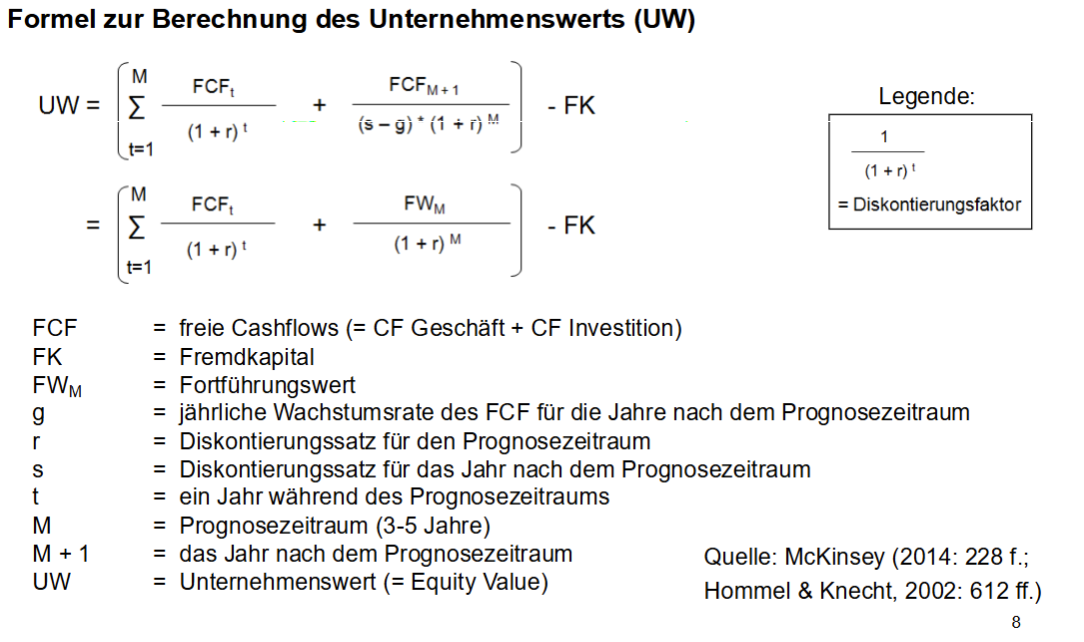
\includegraphics[width=\textwidth,height=0.7\textheight,keepaspectratio]{figures/Formel.png}
     

\section{Managementwissenschaften}
\subsection{Was beeinflusst Erfolg einer Gründung}
Es gibt verschiedene Forschungshypothesen, die recherchiert werden:
\begin{enumerate}
    \item Ebene des Individuums
    \begin{itemize}
        \item Subjektive Merkmale der Gründer sind entscheidend
    \end{itemize}
    \item Geschäftsidee
    \item Kommunikation
    \begin{itemize}
        \item Die Vermittlung/ Kommunikation der Idee ist entscheidend
    \end{itemize}
\end{enumerate}
\subsection{Ethik}
Argumente für das ethische Wesen der Unternehmensgründung 
\begin{itemize}
    \item Inhärent sozial, weil Stakeholder berücksichtig werden müssten
    \item ethisches Potenzial durch Hinterfragung Bestehender Verhältnisse und Lösungsfindung
    \item Trotz Autonomiestreben bestehe ein Verantwortungsgefühl gegenüber Mitarbeitern
\end{itemize}

\subsection{Formen von Unternehmertum}
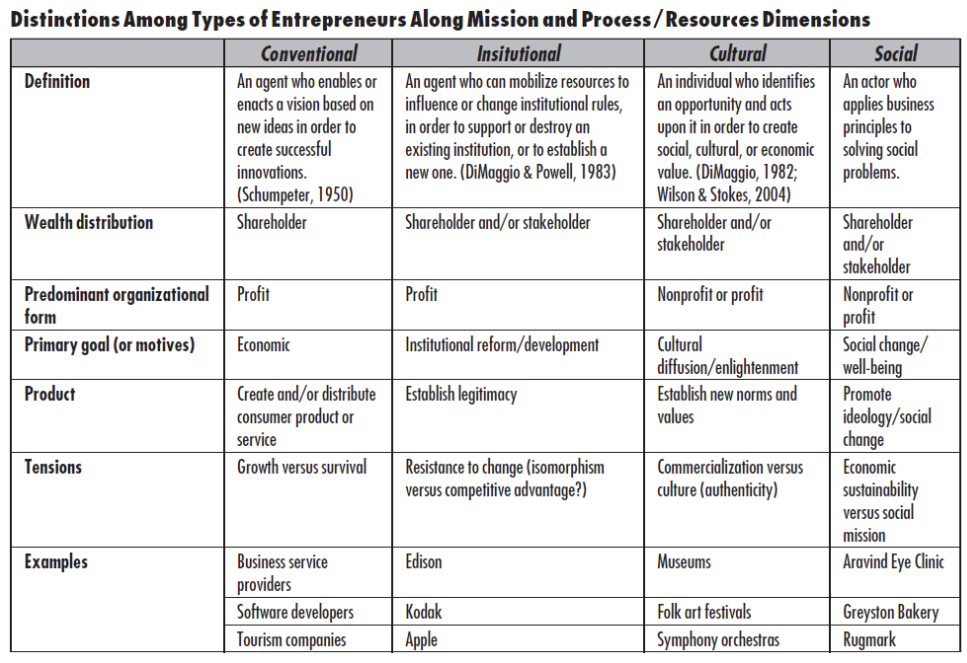
\includegraphics[width=\textwidth,height=0.7\textheight,keepaspectratio]{figures/Formen.png}

\section{Klausurinfos}
Gemäss Kapitel Admin Stuff in BWL Vorlesungsmitschrift und Folien der Übung D.
\end{document}